\documentclass{article}
\usepackage{graphicx} % Required for inserting images

\usepackage{auto-pst-pdf} % Enable PSTricks with pdflatex
% If using Overleaf, the -shell-escape flag is already enabled by default for auto-pst-pdf to work
\usepackage{pst-eucl} % Euclidean geometry

\usepackage{tikz} % ChatGPT likes this for drawing some things
\usetikzlibrary{calc,intersections}

\usepackage{mathtools}


\title{MAT 357-557 Numerical Analysis Project 2}
\author{Austin Zhu, Brillan Morgan, Osprey Varboncoeur}
\date{Spring 2024}

\begin{document}

\maketitle

\section{The Idea}
Our method interpolates between points by interpreting pairs of points as defining circles, then drawing arcs of those circles and finally connecting those arcs with line segments at tangent points.

\subsection{Interpreting the Input Data Set}
For an input data set of \( n \) points, let the \( \frac{n}{2} \) pairs of points be \( P_0, P_1, \ldots, P_{n-2}, P_{n-1} \). Note that \( n \) must be an even number. Let the even-indexed points be the "Control" points, the center points of the circles: \( P_0 = C_0 \), \( P_2 = C_1 \), \( \ldots \), \( P_{n-2} = C_{\frac{n}{2}-1} \). Let the odd-indexed points be the "Anchor" points, the points on the circumference of the circles: \( P_1 = A_0 \), \( P_3 = A_1 \), \( \ldots \), \( P_{n-1} = A_{\frac{n}{2}-1} \). Let each pair of points \( \{C_i, A_i\} \) define a circle:


\vspace{0.2cm} % Adjust the vertical space as needed

\begin{center}
\begin{tikzpicture}
    % Draw the circle
    \draw (0,0) circle (2cm);
    
    % Label the center
    \draw (0,0) node[circle,fill,inner sep=1.5pt,label=below:$C_i$] {};
    
    % Draw a point on the circumference
    \draw (135:2cm) node[circle,fill,inner sep=1.5pt,label=above left:$A_i$] {};
\end{tikzpicture}
\end{center}

\vspace{0.2cm} % Adjust the vertical space as needed

The \( \frac{n}{2} \) pairs of points define \( \frac{n}{2} \) circles. A minimum of four points defining two circles (\( n \geq 4 \)) is required to use our method.

Circles that are adjacent \textit{in the input data set} must be disjoint, that is, they must not intersect or be one inside the other. Circle \( \{C_i, A_i\} \) must be disjoint from circle \( \{C_{i-1}, A_{i-1}\} \), and also disjoint from circle \( \{C_{i+1}, A_{i+1}\} \). Circle \( \{C_i, A_i\} \) may or may not be disjoint from any other circle in the input data set. Note that there are only disjoint-ness requirements for circles based on their positions in the input data set, never based on any geometric relationship.


\subsection{A Parametric, Piecewise Curve}
Let the final curve be defined by a parametic piecewise function of $t$:
\[
\overrightarrow{O}(t) = \overrightarrow{O}_{\lfloor t \rfloor}(t - \lfloor t \rfloor) = \begin{cases}
S_0(t - \lfloor t \rfloor) & \text{for } 0 \leq t - \lfloor t \rfloor < 1, \\
L_1(t - \lfloor t \rfloor) & \text{for } 1 \leq t - \lfloor t \rfloor < 2, \\
R_2(t - \lfloor t \rfloor) & \text{for } 2 \leq t - \lfloor t \rfloor < 3, \\
S_3(t - \lfloor t \rfloor) & \text{for } 3 \leq t - \lfloor t \rfloor < 4, \\
L_4(t - \lfloor t \rfloor) & \text{for } 4 \leq t - \lfloor t \rfloor < 5, \\
R_5(t - \lfloor t \rfloor) & \text{for } 5 \leq t - \lfloor t \rfloor < 6, \\
\vdots & \\
S_{\frac{3n}{2}-3}(t - \lfloor t \rfloor) & \text{for } \frac{3n}{2}-3 \leq t - \lfloor t \rfloor < \frac{3n}{2}-2, \\
L_{\frac{3n}{2}-2}(t - \lfloor t \rfloor) & \text{for } \frac{3n}{2}-2 \leq t - \lfloor t \rfloor < \frac{3n}{2}-1, \\
R_{\frac{3n}{2}-1}(t - \lfloor t \rfloor) & \text{for } \frac{3n}{2}-1 \leq t - \lfloor t \rfloor < \frac{3n}{2}, \\
A_{\frac{n}{2}-1} & \text{for } t = \frac{3n}{2}
\end{cases}
\]

Where:
\begin{itemize}
    \item $\lfloor \cdot \rfloor$ is the floor function, which rounds down to the largest integer value less than or equal to the variable inside. Examples: $\lfloor 2.0 \rfloor = 2.0$, $\lfloor 2.6 \rfloor = 2.0$.
    \item $n$ is the number of points in the input data set
    \item The initial direction of arc travel around circle $\{C_0, A_0\}$ starting from $A_0$ is defined to be counter-clockwise.
    \item $S$ is the "Sender" function that gives the portion of the $\{C_i, A_i\}$ circle's arc which connects its Anchor point $A_i$ to its tangent\footnote{For any two disjoint circles, there exist four tangent lines: two internal tangent lines and two external tangent lines (see Fig.     \ref{fig:external_tangents_only}). For our curve, we will consider only external tangent lines.} "sending" point $T_{iS}$. The sending point is the point on the circle tangent to the line segment connecting circle $\{C_i, A_i\}$ to circle $\{C_{i+1}, A_{i+1}\}$ such that the resulting curve has no corner:
    \begin{itemize}
        \item 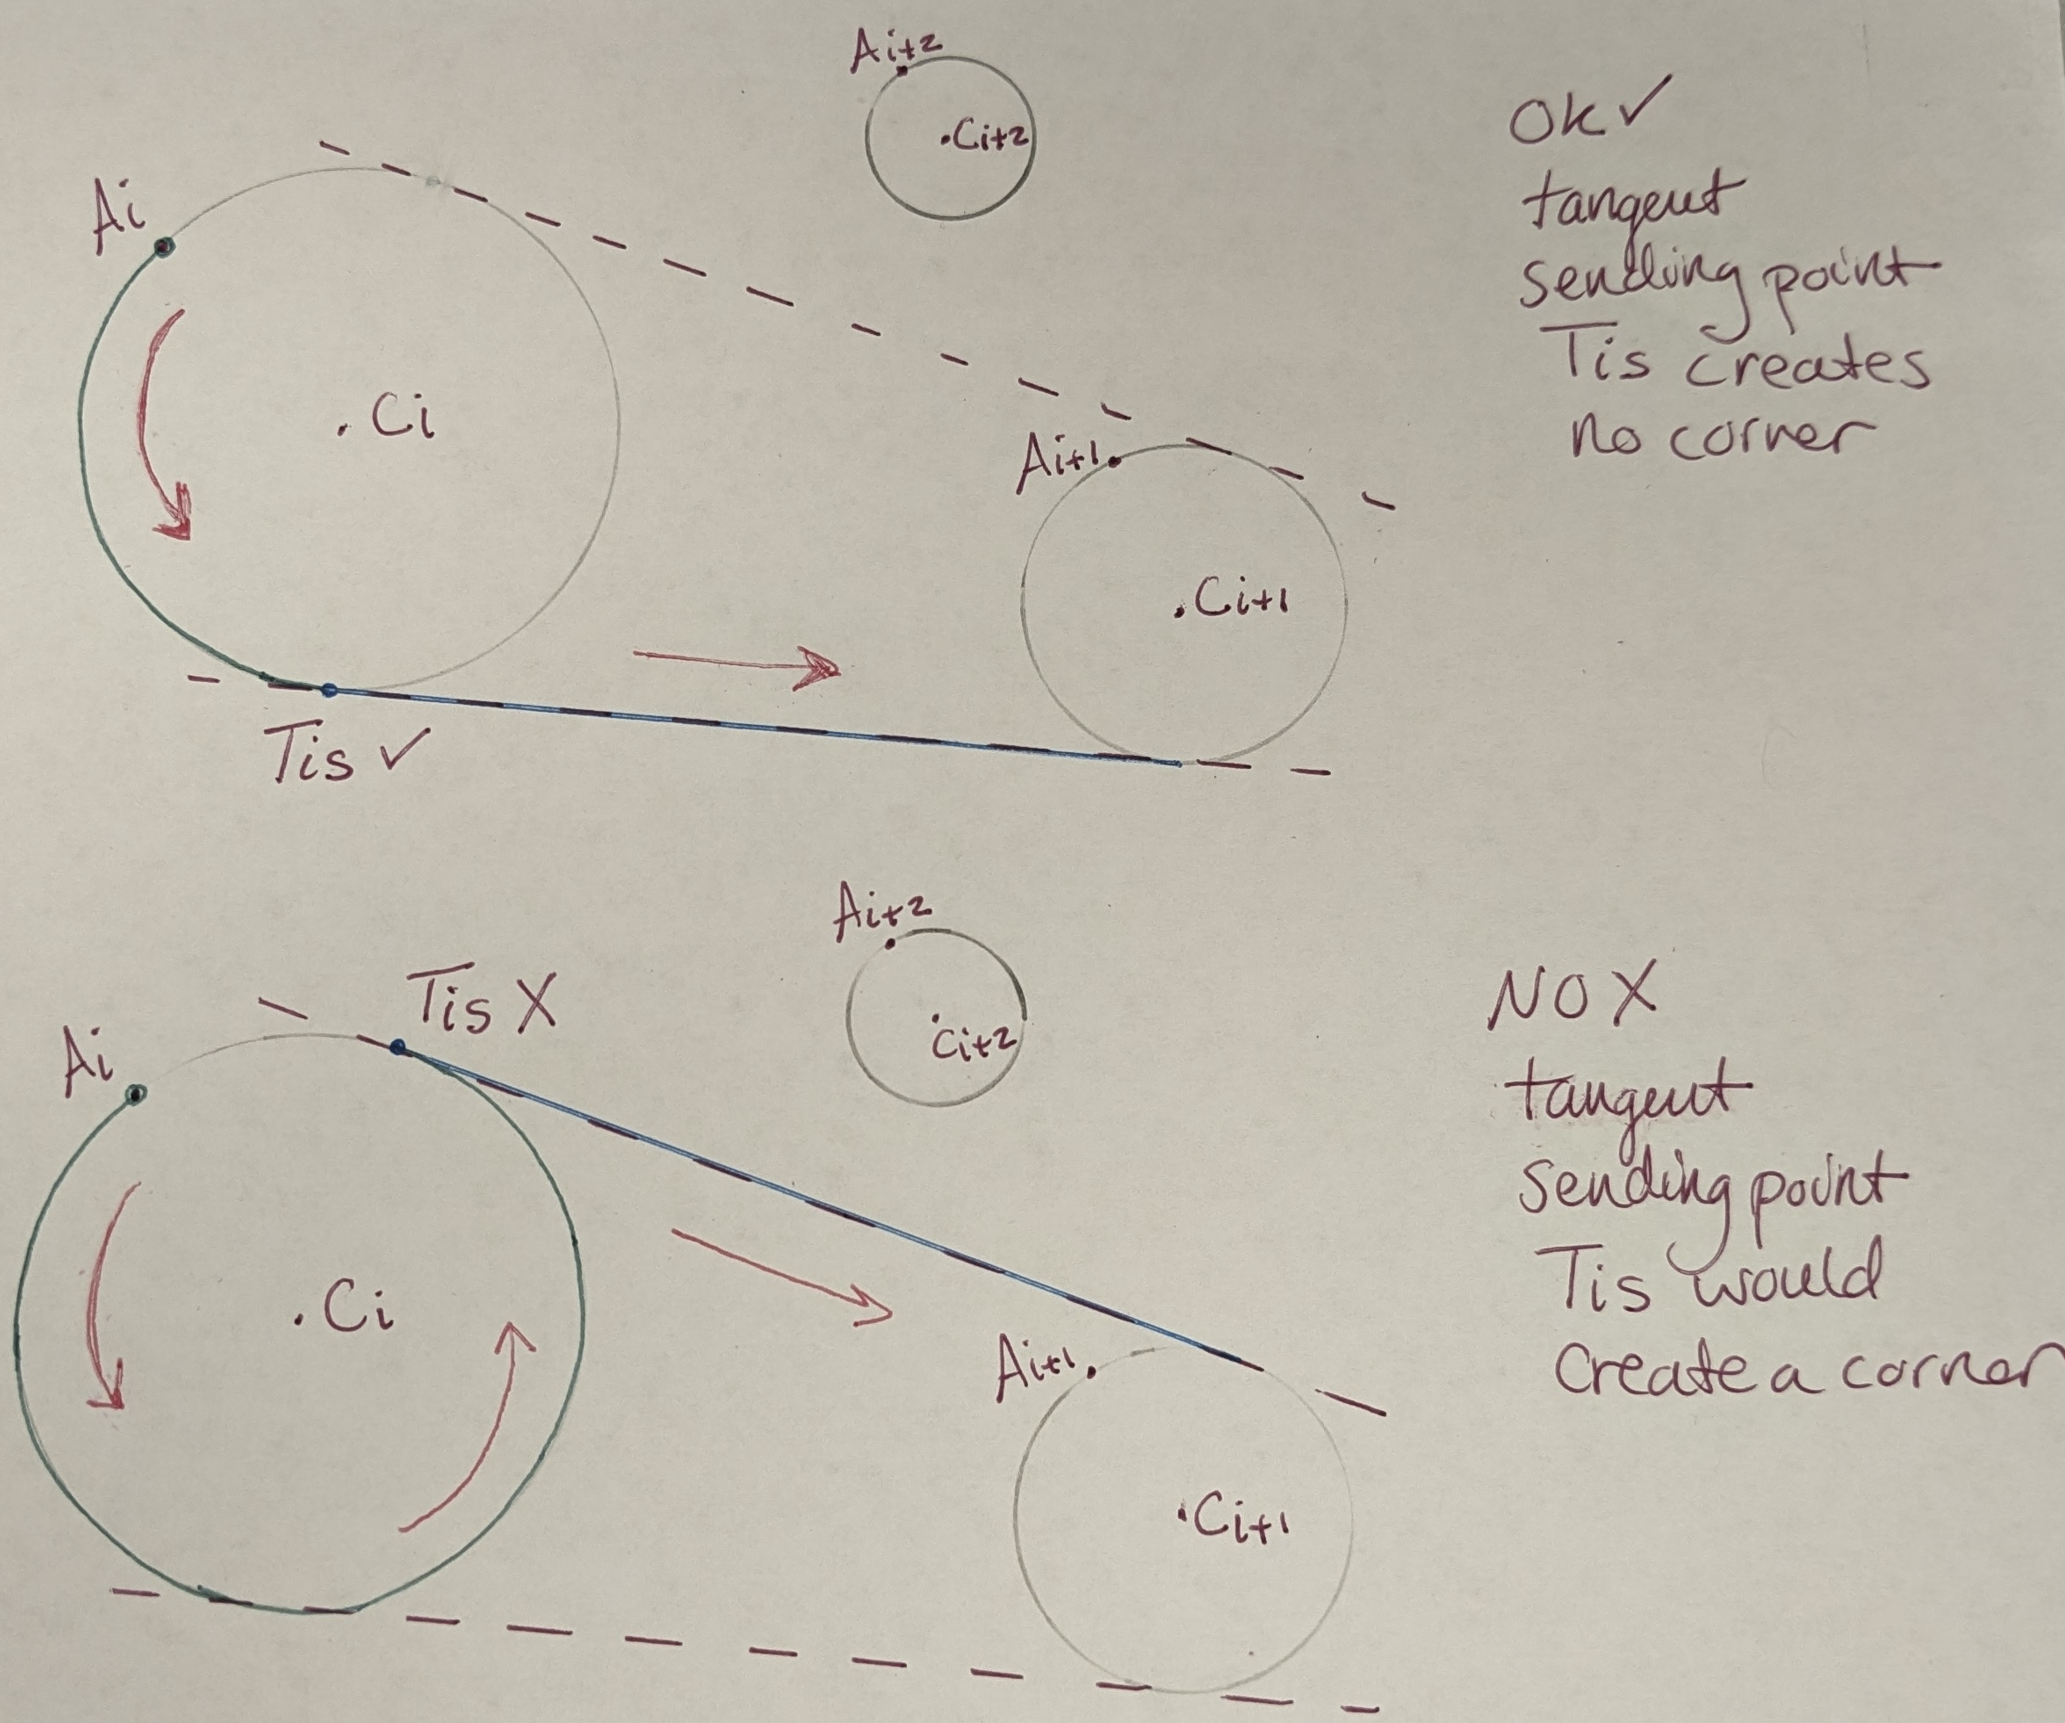
\includegraphics[width=1.0\textwidth]{NoCorner.png}
    \end{itemize}
    Note that the counter-clockwise direction of arc travel specifies which of the tangent points on circle $\{C_i, A_i\}$ will be the correct tangent sending point $T_{iS}$: the one that does not create a corner.
    \item $L$ is the "Line" function that gives the line segment connecting the tangent sending point $T_{iS}$ on circle $\{C_i, A_i\}$ to the tangent receiving point $T_{iR}$ on circle $\{C_{i+1}, A_{i+1}\}$.
    \item $R$ is the "Receiver" function that gives the portion of the $\{C_{i+1}, A_{i+1}\}$ circle's arc that connects its tangent receiving point $T_{iR}$ to its Anchor point $A_{i+1}$.
\end{itemize}
Fig.\ref{fig:SLRExample} shows an example resulting curve with the $S$ "Sending" function plots shown in green, the $L$ "Line" plots shown in blue, and the $R$ "Receiver" plots shown in orange.
\begin{figure}
    \centering
    \includegraphics[width=1.0\textwidth]{FigureXExampleOfSLR_Cropped.png}
    \caption{Example curve showing $S$ "Sending" function plots (green), $L$ "Line" plots (blue), and $R$ "Receiver" plots (orange)}
    \label{fig:SLRExample}
\end{figure}

\begin{figure}[htbp]
    \centering
    %\vspace{0.2cm} % Adjust the vertical space as needed
    \begin{tikzpicture}
        % Draw the larger circle
        \draw (0,0) circle (2cm);
        % Draw the smaller circle
        \draw (5,0) circle (1cm);


        % Tangency points on the larger circle (for reference)
        \coordinate (T1) at (0.4, 1.96);
        \coordinate (T2) at (0.4, -1.96);

        % Tangency points on the smaller circle (for reference)
        \coordinate (T3) at (5.2, 0.98);
        \coordinate (T4) at (5.2, -0.98);

        % Draw the tangent lines (for reference)
        \draw[blue] (T1) -- (T3);
        \draw[blue] (T2) -- (T4);

        % Internal tangency points
        \coordinate (T5) at (1.2, 1.6);
        \coordinate (T6) at (1.2, -1.6);
        \coordinate (T7) at (4.4, 0.8);
        \coordinate (T8) at (4.4, -0.8);

        % Draw the internal tangent lines in red
        \draw[red] (T5) -- (T8);
        \draw[red] (T6) -- (T7);
    \end{tikzpicture}
    \caption{The tangent lines of two disjoint circles: two internal tangent lines (red) and two external tangent lines (blue). Our curve considers only external tangent lines.}
    \label{fig:external_tangents_only}
\end{figure}
%\vspace{0.2cm} % Adjust the vertical space as needed
\subsubsection{Interpretation and Usage of Parameter Variable $t$}
The range of values that can be used with $\overrightarrow{O}(t)$ is $0 \leq t \leq \frac{3n}{2}$. That is, the first point of the curve $P_1 = A_0$ is plotted by function $S_0$ when $t = 0$. The final point of the curve $P_{n-1} = A_{\frac{n}{2}-1}$ is plotted directly when $t = \frac{3n}{2}$, without using any of the $SLR$ functions.
Table \ref{tab:n_t_and_SLR_relationship} gives examples showing the relationship between $n$, the maximum value of $t$, and the indices of all $SLR$ functions (and the final $A$ point) of the piecewise curve definition.

\begin{table}[htbp]
    \centering
    \begin{tabular}{|c|c|c|}
        \hline
        \multicolumn{1}{|c|}{\begin{tabular}[t]{@{}c@{}}
            $n = 4$ points \\
            $\frac{n}{2} = 2$ circles
        \end{tabular}} &
        \multicolumn{1}{c|}{\begin{tabular}[t]{@{}c@{}}
            $n = 6$ points \\
            $\frac{n}{2} = 3$ circles
        \end{tabular}} &
        \multicolumn{1}{c|}{\begin{tabular}[t]{@{}c@{}}
            $n = 8$ points \\
            $\frac{n}{2} = 4$ circles
        \end{tabular}} \\
        \hline
        \multicolumn{1}{|c|}{\begin{tabular}[t]{@{}c@{}}
            $S_0$ \\
            $L_1$ \\
            $R_2$ \\
            $S_3$ \\
            $L_4$ \\
            $R_5$ \\
            $A_1$
        \end{tabular}} &
        \multicolumn{1}{|c|}{\begin{tabular}[t]{@{}c@{}}
            $S_0$ \\
            $L_1$ \\
            $R_2$ \\
            $S_3$ \\
            $L_4$ \\
            $R_5$ \\
            $S_6$ \\
            $L_7$ \\
            $R_8$ \\
            $A_2$
        \end{tabular}} &
        \multicolumn{1}{|c|}{\begin{tabular}[t]{@{}c@{}}
            $S_0$ \\
            $L_1$ \\
            $R_2$ \\
            $S_3$ \\
            $L_4$ \\
            $R_5$ \\
            $S_6$ \\
            $L_7$ \\
            $R_8$ \\
            $S_9$ \\
            $L_{10}$ \\
            $R_{11}$ \\
            $A_3$
        \end{tabular}} \\
        \hline
        \multicolumn{1}{|c|}{\begin{tabular}[t]{@{}c@{}}
            $0 \leq t \leq \frac{3n}{2}$ \\
            \hspace{1.5em}$\leq \frac{3 \cdot 4}{2}$ \\
            $0 \leq t \leq 6$
        \end{tabular}} &
        \multicolumn{1}{|c|}{\begin{tabular}[t]{@{}c@{}}
            $0 \leq t \leq \frac{3n}{2}$ \\
            \hspace{1.5em}$\leq \frac{3 \cdot 6}{2}$ \\
            $0 \leq t \leq 9$
        \end{tabular}} &
        \multicolumn{1}{|c|}{\begin{tabular}[t]{@{}c@{}}
            $0 \leq t \leq \frac{3n}{2}$ \\
            \hspace{1.5em}$\leq \frac{3 \cdot 8}{2}$ \\
            $0 \leq t \leq 12$
        \end{tabular}} \\
        \hline
    \end{tabular}
    \caption{2x4 table with specified content}
    \label{tab:n_t_and_SLR_relationship}
\end{table}

\subsubsection{Counter-clockwise Arc Travel Direction}
For the very start of the curve, we defined the direction of arc travel around circle $\{C_0, A_0\}$ (starting from $A_0$) to be in the counter-clockwise direction.
Defining the travel direction for the first sending arc (on circle $\{C_0, A_0\}$) to be counter-clockwise also defines travel direction for all arcs in the curve to be counter-clockwise.\\ \\

\textbf{DO WE NEED A PROOF FOR THIS?} \\

\subsubsection{Overlapping Arcs}
Consider the scenario where the position of Anchor point $A_{i+1}$ on circle $\{C_{i+1}, A_{i+1}\}$ causes the receiving arc (going from $T_{iR}$ to $A_{i+1}$) to overlap with the sending arc (going from $A_{i+1}$ to $T_{(i+1)S}$). In this scenario, the entire $\{C_{i+1}, A_{i+1}\}$ circle will be plotted. Further, some of circle $\{C_{i+1}, A_{i+1}\}$ will be plotted twice: first by the $R$ function, then again by the $S$ function.\\ \\
\textbf{DIAGRAM TODO}\\ \\
Such overlapping of receiving and sending arcs does not affect which tangent point will become the $T_{(i+1)S}$ tangent sending point for circle $\{C_{i+1}, A_{i+1}\}$. The correct tangent sending point is determined only by the direction of arc travel, which is defined to start as counterclockwise and guaranteed to remain counterclockwise for all arcs in the curve.

\section{The Computation}
Intro to this section to prevent "stacked headings"
\subsection{The Sending Function “S”}

\subsection{The Line Segment Function “L”}

\subsection{The Receiving Function “R”}


\section{Curve Properties}
Our curve connects only the Anchor points from the input data set, that is, the points on the edges of the circles. The Control points serve only to define the center point of each circle. Thus, we have borrowed the point naming convention  of B\'ezier curves.\\
Our curve has no discontinuities or corners. It consists of only circle arcs connected by line segments at mutual tangent points. Since our curve is parametric and not a function of x, it can cross back across where it has already been on the x axis. One nice property of our curve is that it flows pleasingly along its path even though it is made up entirely of simple geometric constructs: circle arcs and line segments.


\section{Explanation}



\section{Analysis}



\section{Further Ideas}
What else we wanted to try
What else we think could be interesting to investigate




\end{document}
